\section{Angriffe}\label{sec:exp_angriffe}

Das Ziel von Differential Privacy in Kombination mit neuronalen Netzen, ist es, Angriffe abzuschwächen. 
Im Folgenden wird anhand zweier Angriffe evaluiert, welchen Effekt die Nutzung von DPSGD hat.
Bei den zwei genutzten Angriffen handelt es sich um die Membership Inference Attacke und die Model Inversion Attacke.

\subsection{Membership Inference Attacke}

Die Membership Inference Attacke soll zeigen, ob ein Datensatz in der Trainingsdatenmenge eines Modells enthalten ist oder nicht.
Dazu werden Shadow Modelle genutzt, welche das anzugreifende Modell nachahmen. 
Die Vorhersagen der Shadow Modelle werden genutzt, um einen Meta-Klassifikator zu trainieren, welcher bestimmt, ob ein Datensatz bei einem Modell zum Training genutzt wurde.

Eine Besonderheit dieses Angriffs ist es, dass sowohl eine Black-Box, als auch eine White-Box Variante möglich ist.
Bei der White-Box Variante kennt der Angreifer die genaue Architektur des anzugreifenden Modells und kann die Architektur der Shadow Modell nachbilden.
In der Black-Box Variante, wird lediglich versucht, ähnliche Architekturen zu kreieren.
Dieses Experiment nutzt den White-Box Ansatz.
Dies liegt daran, dass es bei einem Black-Box Ansatz sein könnte, dass der Angreifer, durch Glück, eine nahezu identische Architektur der Shadow Modelle wählt. 
Somit kann ein Black-Box Ansatz theoretisch genauso effektiv sein, wie der White-Box Ansatz.

\subsubsection*{Membership Inference Attacke gegen das CIFAR-10 Modell}

Die CIFAR-10 Datenmenge besteht bereits aus einer Trainingsdatenmenge und einer Testdatenmenge, welche in Summe aus 60000 Datensätzen bestehen.
Für das Training der Shadow Modelle werden die beiden Datenmengen kombiniert.
Anschließend wird für jedes Shadow Modell zufällig eine Datenmenge, bestehend aus 50000 Datensätzen, für das Training ausgewählt.
Somit dienen die ausgewählten Daten nicht nur für das Training, sondern haben zusätzlich das Label \dq included\dq, wohingegen die nicht ausgewählten Daten das Label \dq excluded\dq\ erhalten.
Die Labels dienen im Anschluss dazu, die Datenmenge für den Meta-Klassifikator zu konstruieren.
Damit die Anzahl der beiden Labels in der Datenmenge gleich ist, werden von der genutzten Trainingsdatenmenge jedes Shadow Modells nur 10000 Datensätze gelabelt.
Somit entstehen pro Shadow Modell 20000 gelabelte Datensätze, jeweils 10000 mit dem Label \dq included\dq\ und 10000 mit dem Label \dq excluded\dq.

Der Meta-Klassifikator ist ein neuronales Netz, welches nur aus vollständig verbundenen Schichten besteht.
Dabei werden 10 Neuronen als Eingabe genutzt, je ein Neuron pro Vorhersagewahrscheinlichkeit einer Klasse, und ein Neuron als Ausgabe, welches das Label \dq included\dq\ oder \dq excluded\dq\ bestimmt.
Die Vorhersagewahrscheinlichkeiten, welche als Eingabe dienen, werden von den Shadow Modellen durch die Softmax-Funktion in den Wertebereich (0,1) übertragen, wobei eine Klasse einen Wert nahe 1 hat, die restlichen Klassen einen Wert von 0.

Die Trainingsdatenmenge und Testdatenmenge des CIFAR-10 Datenbestands könnte genutzt werden, um die Membership Inference Attacke zu bewerten, jedoch haben die Datenmengen eine ungleiche Anzahl an Datensätzen.
Würde der Meta-Klassifikator immer das Label \dq included\dq\ bestimmen, unabhängig des Inputs, dann entspräche dies einer Genauigkeit von \ca 83,3 \%, da die Anzahl der Datensätze in den beiden Datenmengen das gleiche Verhältnis haben.
Deshalb werden aus der Trainingsdatenmenge zufällig 10000 Datensätze ausgewählt. Diese, sowie die 10000 Datensätze der Testdatenmenge, dienen dann zur Evaluierung des Angriffs.
Dazu werden die Datensätze durch das anzugreifende Modell inferiert und die Vorhersagewahrscheinlichkeiten als Eingabe des Meta-Klassifikators genutzt.

Die Modelle, an welchen die Membership Inference Attacke getestet wird, sind die Modelle, welche in Kapitel \ref{sec:hyperparams} trainiert werden.
Dabei wird das beste Modell ohne DPSGD genutzt, sowie jeweils das Modell mit DPSGD, welches mit optimierten Hyperparametern trainiert wurde.

Tabelle \ref{tab:mi_cifar10_base} zeigt die Genauigkeit, welche der Meta-Klassifikator bei der Ausführung der Membership Inference Attacke gegen das CIFAR-10 Modell ohne DPSGD hat.
Dabei wurden eine unterschiedliche Anzahl an Shadow Modellen evaluiert, welche jeweils für 15 Epochen trainiert wurden und dadurch eine ähnliche Genauigkeit wie das originale Modell haben.
Die Genauigkeit des Angriffs ist bei 8,16 und 32 Shadow Modellen ähnlich.
Diese beträgt zwischen 57,4 \% und 58,9 \%.
\begin{table}[!htb]
\centering
\begin{tabular}{|l|l|l|}
\hline
\rowcolor[HTML]{CBCEFB} 
Epsilon & Anzahl Shadow Modelle & Genauigkeit des Angriff \\ \hline
$\infty$ & 8  & 58,0 \% \\ \hline
$\infty$ & 16 & 58,9 \% \\ \hline
$\infty$ & 32 & 57,4 \% \\ \hline
\end{tabular}
\caption{Membership Inference Angriff gegen CIFAR-10 Modell ohne DPSGD}
\label{tab:mi_cifar10_base}
\end{table}

Tabelle \ref{tab:mi_cifar10_part1} zeigt, wie sich die Genauigkeit des Angriffs durch die Nutzung von DPSGD ändert.
Bei allen Modellen mit DPSGD, hat die Membership Inference Attacke eine Genauigkeit zwischen 49,8 \% und 50,2 \%. 
Dadurch ist der Angriff weniger effektiv, als ohne die Nutzung von DPSGD.
\begin{table}[!htb]
\centering
\begin{tabular}{|l|l|l|}
\hline
\rowcolor[HTML]{CBCEFB} 
Epsilon & \begin{tabular}[c]{@{}l@{}}Anzahl \\ Shadow Modelle\end{tabular} & \begin{tabular}[c]{@{}l@{}}Genauigkeit \\ des Angriff\end{tabular} \\ \hline
$\infty$ & 32 & 57,4 \% \\ \hline
1        & 32 & 49,9 \% \\ \hline
5        & 32 & 49,8 \% \\ \hline
10       & 32 & 50,1 \% \\ \hline
20       & 32 & 50,2 \% \\ \hline
30       & 32 & 50,2 \% \\ \hline
50       & 32 & 50,0 \% \\ \hline
\end{tabular}
\caption{Membership Inference Angriff gegen CIFAR-10 Modelle mit DPSGD}
\label{tab:mi_cifar10_part1}
\end{table}

Das Problem des Angriffs ist jedoch, dass dieser nur minimal effektiv gegen ein Modell ohne DPSGD ist. 
Würde der Meta-Klassifikator zufällig ein Label wählen, würde dies einer Genauigkeit von \ca 50 \% entsprechen. 
Gegen ein Modell ohne DPSGD, erreicht der Meta-Klassifkator eine Genauigkeit von bis zu 58,9 \%, was eine Verbesserung ist.
Jedoch ermöglicht dies nicht, eine sachdienliche Aussage zu treffen.
Zusätzlich hat der Angreifer in der Regel keine Möglichkeit, den Angriff zu evaluieren. 
Dies liegt daran, dass der Angreifer keine Informationen \bzgl der genutzten Trainingsdatenmenge hat.
Die geringe Effektivität des Angriffs, sogar in der White-Box Variante, macht die Nutzung von DPSGD entbehrlich.

\subsubsection*{Membership Inference Attacke gegen das ResNet-18 Modell}
Die Membership Inference Attacke wird nur gegen das ResNet-18 Modell evaluiert, jedoch nicht gegen das Vision Transformer Modell.
Dies liegt an den benötigten Ressourcen, eine Vielzahl an Shadow Modellen zu trainieren, welche jeweils die Vision Transformer Architektur nutzen.

Das ResNet-18 Modell erkennt 40 Merkmale anhand von Gesichtsbildern des CelebA Datenbestand.
Im Gegensatz zu dem CIFAR-10 Modell wird nicht eine Klasse vorhergesagt, sondern 40 unabhängige Merkmale.
Dabei handelt es sich um eine sogenannte Multi-Label Klassifizierung, also einer Klassifikation bei welcher mehrere Labels vorhergesagt werden können.
Für das Modell sind diese 40 Labels unabhängig, fachlich sind jedoch einige dieser Labels verbunden.
So gibt es beispielsweise unterschiedliche Labels, welche für unterschiedliche Haarfarben stehen.
Da jede Person in dem Datenbestand eine Haarfarbe hat, hat maximal eines der Haarfarben-Labels den Wert 1, wohingegen die restlichen Haarfarben den Wert 0 haben.

Die Membership Inference Attacke gegen die ResNet-18 Modelle werden simultan zu den Angriffen gegen die CIFAR-10 Modelle durchgeführt.
Tabelle \ref{tab:mi_resnet18} zeigt die Genauigkeit des Angriffs gegen Modelle mit einem unterschiedlichen $\epsilon$-Wert.
Es wurden jeweils 8 Shadow Modelle trainiert und zum Labeln genutzt.
Der Angriff gegen das Modell ohne DPSGD hat eine Genauigkeit von 52,1 \% und ist damit nur minimal besser, als bei einer zufälligen Vorhersage.
Gegen Modelle die DPSGD benutzten ist der Angriff noch weniger effektiv und erreicht eine Genauigkeit von maximal 50,6 \%.

\begin{table}[!htb]
\centering
\begin{tabular}{|l|l|}
\hline
\rowcolor[HTML]{CBCEFB} 
Epsilon  & Genauigkeit des Angriff \\ \hline
$\infty$ & 52,1 \%                 \\ \hline
1        & 50,2 \%                 \\ \hline
5        & 50,6 \%                 \\ \hline
10       & 50,1 \%                 \\ \hline
\end{tabular}
\caption{Membership Inference Angriff gegen ResNet-18 Modelle mit DPSGD}
\label{tab:mi_resnet18}
\end{table}

\subsection{Model Inversion Attacke}

Bei der Model Inversion Attacke werden die Ausgaben eines Modells genutzt, um Rückschlüsse zu den Trainingsdaten zu ziehen.
Der hier evaluierte Angriff wird auch Reconstruction Attacke genannt. 
Ziel ist es, einen Datensatz aus dem Trainingsdatenbestand nachzubilden, lediglich anhand des Modells.
Hierfür wird ein Startbild in das Modell gegeben, welches zu Beginn lediglich eine Ansammlung von zufälligen Pixeln ist.
Die Vorhersage des Modells wird anschließend mit einer Verlustfunktion durch das Modell backpropagiert, jedoch werden nicht die Gewichte des Modells angepasst, sondern die Werte des Startbildes.
Dadurch verändert sich das Bild, bis es das gewünschte Label zeigt.
Der Vorgang wird dabei iterativ wiederholt.
Zusätzlich wird in jedem Schritt das Bild mittels eines Autoencoders entrauscht, sodass sich die zufällige Ansammlung von Pixeln zu einem möglichst realistischen Bild umwandeln.
Der iterative Vorgang kann nach einer festgelegten Anzahl an Wiederholungen gestoppt werden, oder bis das rekonstruierte Bild den gewünschten Detailgrad erreicht hat.

\subsubsection*{Model Inversion Attacke gegen CIFAR-10 Modell}
Um die Model Inversion Attacke durchzuführen, wurde zu Beginn ein Autoencoder trainiert.
Dieser soll Bilder entrauschen, \dahe das Rauschen aus Bildern entfernen und diese realistischer werden lassen.
Als Ausgabe des Modells werden daher die Bilder des CIFAR-10 Trainingsdatenbestand genutzt, wobei die Eingabe jeweils eine verrauschte Version dieses Bildes ist.
Die verrauschten Bilder können erzeugt werden, indem ein zufälliges Rauschen über jedes Pixel hinzugefügt wird.

Der Autoencoder hat die gleiche Eingabedimension wie Ausgabedimension, welche $32\times32\times3$ Pixeln entspricht.
In einer verdeckten Schicht ist die Dimension jedoch niedriger, welche dafür sorgt, dass das Modell in dieser nur einen Teil der Bildinformationen zwischenspeichern kann.
Zum Verkleinern der Dimensionen werden Faltungsschichten und Pooling-Operationen genutzt.
Das Vergrößern der Dimension wird mit transponierten Faltungsschichten ausgeführt.
Transponierte Faltungsschichten funktionieren simultan zu normalen Faltungsschichten, jedoch wird zuvor das Bild um interpolierte Pixel erweitert. 
Abbildung \ref{fig:autoencoder_cifar} zeigt, welchen Effekt der Autoencoder auf verrauschte Bilder ausübt.
Der linke Teil der Abbildung zeigt ein originales Bild aus der CIFAR-10 Datenmenge. 
Dieses ist der Klasse \dq Schiff\dq\ untergeordnet.
Der mittlere Teil der Abbildung zeigt dabei die zufällig verrauschte Version dieses Bildes.
Das Schiff ist dabei kaum zu erkennen, da viele Pixel des Bildes eine andere Farbe angenommen haben.
Der rechte Teil der Abbildung zeigt, wie die Ausgabe des Autoencoders bei Eingabe des verrauschten Bildes aussieht.
Das Schiff ist wieder erkennbar und das Bild ähnelt dem originalen Bild.

\begin{figure}[!htb]
\centering
\begin{subfigure}[h]{0.3\textwidth}
  \centering
  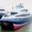
\includegraphics[width=\linewidth]{figures/autoencoder_cifar/1.jpg}
  \caption{Originales Bild}
\end{subfigure}
\begin{subfigure}[h]{0.3\textwidth}
  \centering
  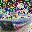
\includegraphics[width=\linewidth]{figures/autoencoder_cifar/2.jpg}
  \caption{Verrauschtes Bild}
\end{subfigure}
\begin{subfigure}[h]{0.3\textwidth}
  \centering
  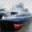
\includegraphics[width=\linewidth]{figures/autoencoder_cifar/3.jpg}
  \caption{Ausgabe Autoencoder}
\end{subfigure}
\caption{Autoencoder CIFAR-10 Datenbestand}
\label{fig:autoencoder_cifar}
\end{figure}

Wird die Model Inversion Attacke gegen das CIFAR-10 Modell ohne DPSGD ausgeführt, kann kein Bild rekonstruiert werden.
Parameter wie der Optimizer, die Lernrate oder die Verlustfunktion wurden angepasst, jedoch führte dies zu keiner Verbesserung des Angriffs 
Zusätzlich wurden unterschiedliche Methoden der Initialisierung des Startbildes gewählt.
Ebenfalls wurden evaluiert, den Angriff einige Iterationen ohne den Autoencoder durchzuführen.
Keine der Anpassungen sorgte für eine Verbesserung des Angriffs.

Abbildung \ref{fig:moder_inv_c10} zeigt, das Ergebnis einer Model Inversion Attacke, wenn ein Bild mit dem Label \dq Schiff\dq\ nachgebildet werden soll.
Das linke Bild entspricht dem initialen Startbild, bei dem alle Farbwerte jeweils mit dem Wert 0,5 befüllt werden. 
Dies entspricht einem grauen Bild.
Das mittlere Bild zeigt, wie sich das Bild nach einigen Iterationen des Angriffs ohne Autoencoder verändert hat.
Dabei handelt es sich um zufällig aussehende Pixel, jedoch sagt das CIFAR-10 Modell bei diesem Bild das gewünschte Label \dq Schiff\dq\ vorher.
Das rechte Bild zeigt das Ergebnis des Angriffs, nachdem das Bild für weitere Iterationen angepasst wurde und pro Iteration mit dem Autoencoder angepasst wurde.
Das entstandene Bild besteht primär aus gräulichen Pixeln, welche eine Musterung aufweisen, die vermutlich vom Autoencoder stammt.
Es ist kein Schiff zu erkennen.
\begin{figure}[!htb]
\centering
\begin{subfigure}[h]{0.3\textwidth}
  \centering
  
\includegraphics[width=\linewidth]{figures/autoencoder_cifar/mi_cifar_start_grey.jpg}
  \caption{Initiales Bild\\jeder Wert=0,5}
\end{subfigure}
\begin{subfigure}[h]{0.3\textwidth}
  \centering
  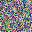
\includegraphics[width=\linewidth]{figures/autoencoder_cifar/mi_cifar_mid_grey.jpg}
  \caption{Anpassung \\ohne Autoencoder}
\end{subfigure}
\begin{subfigure}[h]{0.3\textwidth}
  \centering
  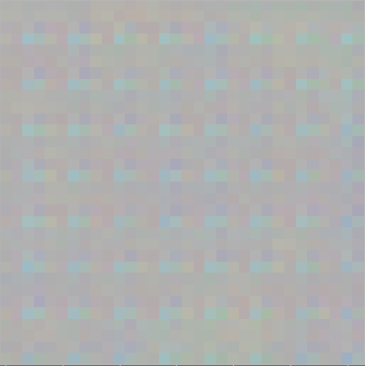
\includegraphics[width=\linewidth]{figures/autoencoder_cifar/mi_cifar_finish_grey.png}
  \caption{Anpassung \\mit Autoencoder}
\end{subfigure}
\caption{Model Inversion Attacke gegen CIFAR-10}
\label{fig:moder_inv_c10}
\end{figure}

\subsubsection*{Model Inversion Attacke gegen ResNet-18 Modell}

Die Model Inversion Attacke gegen das ResNet-18 Modell erfolgt simultan zu der Attacke gegen das CIFAR-10 Modell.
Zuerst wird ein Autoencoder trainiert, welcher das Rauschen von Bildern der CelebA Datenmenge entfernt.
Abbildung \ref{fig:autoencoder_celeba} zeigt, wie ein verrauschtes Bild mittels des Autoencoders wieder entrauscht werden kann.
Der Output des Autoencoders, also das entrauschte Bild, zeigt das Gesicht einer Person, jedoch ist das Bild weniger scharf als das originale Bild.

\begin{figure}[!htb]
\centering
\begin{subfigure}[h]{0.3\textwidth}
  \centering
  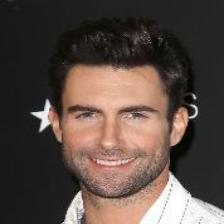
\includegraphics[width=\linewidth]{figures/autoencoder_r18/faces_autoencoder1.jpg}
  \caption{Originales Bild}
\end{subfigure}
\begin{subfigure}[h]{0.3\textwidth}
  \centering
  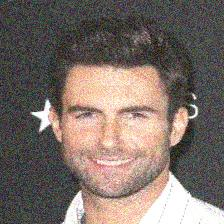
\includegraphics[width=\linewidth]{figures/autoencoder_r18/faces_autoencoder2.jpg}
  \caption{Verrauschtes Bild}
\end{subfigure}
\begin{subfigure}[h]{0.3\textwidth}
  \centering
  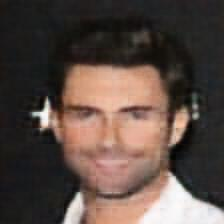
\includegraphics[width=\linewidth]{figures/autoencoder_r18/faces_autoencoder3.jpg}
  \caption{Ausgabe Autoencoder}
\end{subfigure}
\caption{Autoencoder CelebA Datenbestand}
\label{fig:autoencoder_celeba}
\end{figure}

Die Model Inversion Attacke ist ebenfalls gegen das ResNet-18 Modell ohne DPSGD nicht effektiv.
Abbildung \ref{fig:moder_inv_cr18} zeigt dabei das Ergebnis einer Rekonstruktion. 
Die Labels, nach welchen das Bild rekonstruiert werden soll, entstammen dem Beispielbild aus Abbildung \ref{fig:autoencoder_celeba}.
Als Startbild dient hier wieder ein Bild, bei welchem jeder Farbwert auf den Wert 0,5 gesetzt ist.
Dieses wurde für einige Iterationen durch die Backpropagation des Modells angepasst, jedoch vorerst ohne Autoencoder.
Hier entsteht eine zufällige Ansammlung an Pixeln, welche jedoch vom Modell die gewünschten Labels vorhergesagt bekommt.
Nach einigen weiteren Iterationen, sowie zusätzlichen Anpassungen mittels des Autoencoders, entsteht wieder ein relativ gräuliches Bild.
Dieses besitzt ebenfalls eine Musterung, welche vermutlich durch den Autoencoder entstanden ist.
\begin{figure}[!htb]
\centering
\begin{subfigure}[h]{0.3\textwidth}
  \centering
  
\includegraphics[width=\linewidth]{figures/autoencoder_r18/faces_mi1.jpg}
  \caption{Initiales Bild\\jeder Wert=0,5}
\end{subfigure}
\begin{subfigure}[h]{0.3\textwidth}
  \centering
  
\includegraphics[width=\linewidth]{figures/autoencoder_r18/faces_mi2.jpg}
  \caption{Anpassung ohne\\Autoencoder}
\end{subfigure}
\begin{subfigure}[h]{0.3\textwidth}
  \centering
  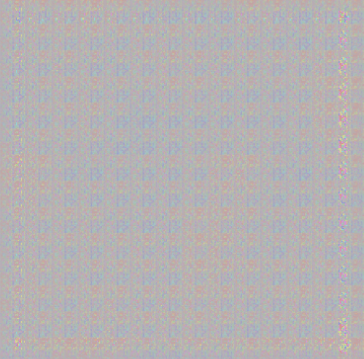
\includegraphics[width=\linewidth]{figures/autoencoder_r18/faces_mi3.png}
  \caption{Anpassung mit\\Autoencoder}
\end{subfigure}
\caption{Model Inversion Attacke gegen ResNet-18 Modell}
\label{fig:moder_inv_cr18}
\end{figure}